\chapter{%
論文の体裁}

前章では,
研究内容を論文化する際にどのような論理構造に当てはめていけばよいかを述べた.
本章では,
文章の体裁の標準化について考察する.


\section{\LaTeX の使用}

原則として \LaTeX を使用すること.
本手引を \LaTeX のテンプレートとして使えば,かなり整った論文になるはずである.
ワード等のワープロソフトを使用するのは,
目次,章番号,式番号,図表番号,参考文献等の参照などの変更の手間,数式の美しさ,
機種やバージョンに依存する互換性,などに問題があることから推奨しない.


\section{和文と英文の混用}

論文中では,和文と英文が共に使用されるため,
読みやすい文にするには注意が必要である.


\subsection{英語の使用}

本文中に英語(カタカナ語)がいきなり出てきていないかチェックすること.
日本語で論文を書く場合,日本語で書けるものは日本語で書くのが原則である.
慣用的に英語での表現が主流のもの,英語でしか表現できないもののみを英語で記述する.


\subsection{句読点}

和文の句読点は,全角の ``\makebox[1zw][c]{,}'' と ``\makebox[1zw][c]{.}''
を使用し ``\makebox[1zw][c]{、}'' と ``\makebox[1zw][c]{。}'' は使用しないこと.
同様に,
欧文中では欧文半角の ``,'' と ``.'' を使うこと.


\subsection{括弧}

和文中では全角の括弧()を使用する.
欧文中では半角の括弧 () を使用する.


\section{段落}

各段落の最初は全角1字分(2字分ではない)だけ空白を入れる.
段落の終わり以外では改行しないこと.

段落最初の空白は,このテンプレートを使えば自動的に挿入される.


\section{参考文献}

「参考文献」は特に日本語と英語が混じり合うので,句読点,スペースなどに注意すること.
記述は,本稿のフォーマットに従うように.
すなわち,
和文成書の場合 \Cite{jbook},
和文論文の場合 \Cite{jpaper},
英文成書の場合 \Cite{ebook},
英文論文の場合 \Cite{epaper},
となる.
これは,
日本ロボット学会誌の参考文献のフォーマットを多少改変したものである.

英文著者名のイニシャル内には,省略のピリオドがあってもスペースは不要であるが,
イニシャルとファミリーネームの間には,
半角スペースが必要である.
例えば M.W.{\textvisiblespace}Spong{\textvisiblespace}and{\textvisiblespace}O.{\textvisiblespace}Khatib:{\textvisiblespace}``...,'' のようになる.

文献タイトルのあとのコンマの位置は和文の場合 ``...'',となるが,
欧文の場合は ``...,'' のように中に記述する.


\section{記号}

使用する記号のすべてについて,
最初に出てきた時に,その定義ないし説明が与えられているかどうかをチェックすること.
また同じ記号が異なる意味で使われていないことを確認すること.


\section{数式}

線形代数には不可欠な,スカラー,ベクトル,行列の区別を明確にすること.
スカラーを表わす変数なら $x$ のように通常の Roman のイタリック体,
ベクトルなら $\bm{x}$ のように Bold の小文字,
行列なら $\bm{X}$ のように Bold の大文字で表現するのが慣例である.

また,$\sin$ などのあらかじめ定められた関数は $sin$ としないこと.
例えば $sinhx$ などとしてしまうと,
三角関数 $\sin hx$ なのか双曲線関数 $\sinh x$ なのか判別不能である.
文章についてもそうであるが,
数式はなおさら一意に解釈できるように気を配ること.
これは $\cos$,$\tan$,$\atan$,$\diag$,$\rank$ なども同様である.

数式の記述例を付録に示すので参照のこと.


\begin{table}[t]
	\caption{二自由度マニピュレータ軌道制御シミュレーションのパラメータ}							\label{table:c3/parameters}
	\begin{center}
		\small
		\begin{tabular}{|c|c|c|c|c|c|}																								\hline
			リンク		& リンク長	& リンク			& リンク		& リンク					& 関節							\\
			\&			&			& 重心位置			& 質量			& 慣性モーメント			& ダンパ係数					\\
			joint $i$	& $l_i$ [m]	& $l_\mi{gi}$ [m]	& $m_i$ [kg]	& $I_i$ [kg$\cdot$m${}^2$]	& $d_i$ [N$\cdot$m$\cdot$s/rad]	\\ \hline
			1			& 0.5000	& 0.2500			& 3.000			& 0.2458					& 0.1000						\\
			2			& 0.5000	& 0.3125			& 4.000			& 0.2927					& 0.1000						\\ \hline
        \end{tabular}
    \end{center}
\end{table}


\section{図表}

図や表は本文中で必ず引用されており,
その図や表の説明や見方が本文中で記述されていること.
またその図や表から得られる結論(結果)が記述されており,
図や表が複雑な場合には,
そのどの部分に注目すればそのような結論が得られるかが記述されていること.
定義のなされていない記号が図や表中にないかどうかチェックすること.

グラフについては,
曲線の区別が必要な場合は区別のつきやすい線種(実線と破線など.点線は時々区別しがたいことがある)を使用すること.
また縦軸と横軸の説明と単位が記入されていることをチェックすること.
単位は特に重要であるので必ず書く.単位が無い場合も [-] として無次元数であることを明示する.

グラフを書く際には,グラフ描画ソフトウェアのデフォルト設定を何も考えずに踏襲することは厳禁である.
グラフで伝えたい内容の意味を考え,必要十分な記述を心掛けよ.
具体的注意点は,文献 \Cite{04} の第4章「図の作成法と作図力学」に詳しい.

最近目につくのは,エクセルのデフォルト設定の「グレーでの背景塗りつぶし」と「横線のみの実線のグリッド線」を変更せずにグラフを書く例である.
コントラストを考えればグレーで背景を塗りつぶす意味はなく,白背景にすべきである.
また,縦軸と横軸の両方が離散的でなく連続的な数値を取りうるデータを扱うグラフの場合には,
グリッド線は縦横格子状に書くべき(後述の \Fig{c3/SVsWF} 参照)である.
また,グリッド線は補助線であるので,原則として点線にすべきである.

キャプションは,図・グラフの場合は下部に,表の場合は上部に置く.
また,図表内のテキスト,およびキャプションは英語で記述する例が多いが,
日本語で書く修論・卒論では,日本語で書いてもよいであろう.
キャプションには,その図表の内容を端的に表わすタイトルを書くこと.
単なる「実験システム」とするのではなく,
例えば,後述の \Fig{c3/system} のキャプションのように,
何を実験するシステムなのかを記述すること.

グラフのキャプションで注意すべきは,意味のない記述である.
例えば,横軸を電圧,縦軸を電流として描画したグラフのキャプションを「電圧と電流の関係」としてしまうことである.
これはグラフを見れば分かる情報を単に書き直しただけであり,あまりにも陳腐である.


\begin{figure}[b]
	\setlength{\unitlength}{1mm}
	\begin{center}
		\begin{picture}(43,34)
%			\put( 0.0,  0.0){\framebox(43,30)}
			\put( 0.0,  0.0){\makebox(0,0)[lb]{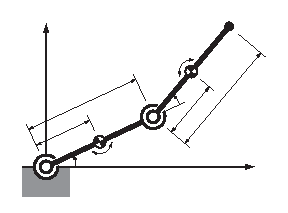
\includegraphics{Fig_c3/manipulator.eps}}}
			\put( 1.0,  7.0){\makebox(0,0)[c] {\tiny $\Sigma_R$}}
			\put(41.0,  4.0){\makebox(0,0)[c] {\tiny $x$}}
			\put( 3.0, 28.0){\makebox(0,0)[c] {\tiny $y$}}
			\put(10.0, 18.0){\makebox(0,0)[c] {\tiny $l_1$}}
			\put(37.0, 15.0){\makebox(0,0)[c] {\tiny $l_2$}}
			\put(15.0, 13.5){\makebox(0,0)[c] {\tiny $l_\mi{g1}$}}
			\put(34.0, 20.0){\makebox(0,0)[c] {\tiny $l_\mi{g2}$}}
			\put(16.5,  7.0){\makebox(0,0)[l] {\tiny $m_1$, $I_1$}}
			\put(27.0, 23.0){\makebox(0,0)[r] {\tiny $m_2$, $I_2$}}
			\put(12.0,  3.0){\makebox(0,0)[c] {\tiny $\theta_1$}}
			\put(29.5, 17.5){\makebox(0,0)[c] {\tiny $\theta_2$}}
			\put(38.0, 30.0){\makebox(0,0)[l] {\tiny $\bm{r}=[r_x,\,r_y]^T$}}
		\end{picture}
	\end{center}
	\vspace{-5mm}	% 美的センスによって適当に設定
	\caption{平面二自由度マニピュレータのモデル}													\label{fig:c3/manipulator}
\end{figure}


\subsection{図表の記述例}

表,図(イラスト),図(グラフ)の例をそれぞれ,
\Table{c3/parameters},\Fig{c3/manipulator},\Fig{c3/SVsWF} に示す.

\begin{figure}[b]
	\setlength{\unitlength}{1mm}
	\begin{center}
		\begin{tabular}{cc}
			\begin{picture}(60,55)
%				\put( 0.0, 0.0){\framebox(60,55)}
				\put(55.0, 4.0){\makebox(0,0)[rb]{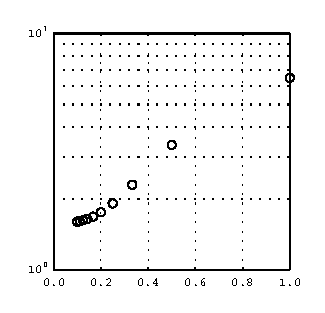
\includegraphics{Fig_c3/SVsWF_long.eps}}}
				\put(60.0, 0.0){\makebox(0,0)[rb]{\scriptsize $1/n_\mi{vj}$ [-]}}
				\put( 0.0,28.0){\makebox(0,0)[l] {\rotatebox{90}{\scriptsize average of $\sigma_1$ [m/s${}^2$]}}}
			\end{picture} &
			\begin{picture}(60,55)
%				\put( 0.0, 0.0){\framebox(60,55)}
				\put(55.0, 4.0){\makebox(0,0)[rb]{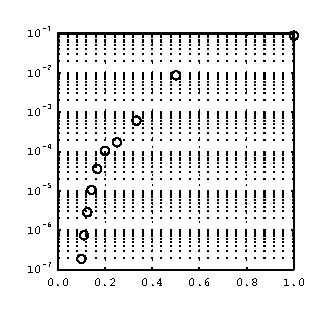
\includegraphics{Fig_c3/SVsWF_short.eps}}}
				\put(60.0, 0.0){\makebox(0,0)[rb]{\scriptsize $1/n_\mi{vj}$ [-]}}
				\put( 0.0,28.0){\makebox(0,0)[l] {\rotatebox{90}{\scriptsize average of $\sigma_2$ [m/s${}^2$]}}}
			\end{picture} \\
			{\footnotesize (a) 長軸の長さ} &
			{\footnotesize (b) 短軸の長さ}
		\end{tabular}
	\end{center}
	\vspace{-3mm}	% 美的センスによって適当に設定
	\caption{動的可操作性楕円体の軸長(特異値)の変化}												\label{fig:c3/SVsWF}
\end{figure}

図表を \LaTeX のコード上でいかに表現するかは各個人によって様々な技術があり,
どれを使えば良いかは各自が判断すること.
著者は,基本的に例示したような方法で表現している.
特徴は,テキストを図のファイル中に書くのではなく,
\texttt{picture} 環境を使ってソースコードの中で記述していることである.
これによって,
\begin{itemize}
	\item 本文と図の数式の体裁の完全な一致
	\item ソースコードでのスペルチェック
\end{itemize}
が可能になる.
しかし,非常に手間がかかるのであまりお勧めできる方法ではない.
一般的な方法でもないので必ずしも真似をする必要はないことに注意されたい.

最後に,シンプルなコードの例として,写真を \Fig{c3/system} に示す.

\begin{figure}[b]
	\vspace{10mm}	% 美的センスによって適当に設定
	\begin{center}
		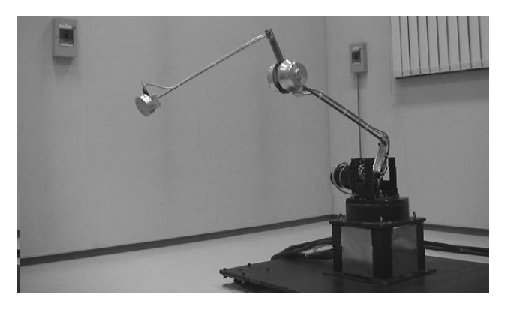
\includegraphics{Fig_c3/image_08.eps}
	\end{center}
	\vspace{-3mm}	% 美的センスによって適当に設定
	\caption{動的可操作性楕円体計測実験システム}													\label{fig:c3/system}
\end{figure}
